\documentclass[a4paper,12pt]{article}
\usepackage{maratona_template}
\usepackage[T1]{fontenc}

\thispagestyle{empty}

\newtheorem{propriedade}{Propriedade}
\newtheorem{definicao}{Definição}

\begin{document}

\begin{center}
\Large{INSTITUTO FEDERAL DO SUL DE MINAS GERIAS}\\
\large{Campus Poços de Caldas}\\
\vspace{10cm}
\Large{Notebook para as Maratonas de Programação}\\
\large{Equipe SK Teletom}
\end{center}

\newpage
\tableofcontents
\thispagestyle{empty}

\newpage
\section{Template}
\inserircodigo{c++}{template.cpp}{8}{8}{}

\newpage
\section{Matemática}
\subsection{Divisão de números inteiros com resto negativo}

Caso seja necessário dividir números inteiros com resto um resto que possivelmente negativo

\inserircodigo{c++}{matematica/div_numeros_inteiros_resto_negativo.cpp}{8}{8}{}

\subsection{Condição existência e classificação de triângulo}

Para um triângulo existir, as três condições devem ser satisfeitas.

\inserircodigo{c++}{matematica/condicao_existencia_triangulo.cpp}{8}{8}{}

\subsection{Comparação entre 2 valores tipo Double}

A comparação entre dois doubles pode retornar valores indejados. Por isso uma função especial para comparação pode ser necessária.

\inserircodigo{c++}{matematica/comparacao_double.cpp}{8}{8}{}

\subsection{Primo rápido – O($\surd$n)}

\inserircodigo{c++}{matematica/primo_rapido_sqrt_n.cpp}{8}{8}{}

\subsection{Crivo de Erastótenes}

\inserircodigo{c++}{matematica/crivo_erastotenes.cpp}{8}{8}{}

\subsection{Checar se um dado bit está ligado}

\inserircodigo{c++}{matematica/check_bit_is_set.cpp}{8}{8}{}

\subsection{Extrair o bit menos significante}

\inserircodigo{c++}{matematica/get_lsb.cpp}{8}{8}{}

\subsection{Contar o número de bits iguais a 1}

\inserircodigo{c++}{matematica/contar_bits_iguais_1.cpp}{8}{8}{}

\subsection{Checar se um número é potência de 2}

\inserircodigo{c++}{matematica/check_is_power_2.cpp}{8}{8}{}

\subsection{Ligar um bit em um número}

\inserircodigo{c++}{matematica/liga_bit_em_numero.cpp}{8}{8}{}

\subsection{Desligar o bit}

\inserircodigo{c++}{matematica/desliga_bit.cpp}{8}{8}{}

\subsection{OR nos Bits ( | )}

\inserircodigo{c++}{matematica/or_nos_bits.cpp}{8}{8}{}

\subsection{AND nos bits (\&)}

\inserircodigo{c++}{matematica/and_nos_bits.cpp}{8}{8}{}

\subsection{XOR nos bits (\textsuperscript{$\wedge$})}

\inserircodigo{c++}{matematica/xor_nos_bits.cpp}{8}{8}{}

\subsection{Shift Esquerdo ( << )}

\inserircodigo{c++}{matematica/shift_esq.cpp}{8}{8}{}

\subsection{Shift Direito ( >> )}

\inserircodigo{c++}{matematica/shift_dir.cpp}{8}{8}{}

\subsection{Arredondamento para cima}

\inserircodigo{c++}{matematica/arrendondamento_cima.cpp}{8}{8}{}

\subsection{Número de casas decimais de um número}

\inserircodigo{c++}{matematica/num_casas_decimais_num.cpp}{8}{8}{}

\subsection{Zerar conteúdo de um array 2d}

\inserircodigo{c++}{matematica/zera_conteudo_array_2d.cpp}{8}{8}{}

\subsection{Zerar conteúdo de um array 1d}

\inserircodigo{c++}{matematica/zera_conteudo_array_1d.cpp}{8}{8}{}

\subsection{Cuidado para divisão de dois floats ou double}

\inserircodigo{c++}{matematica/div_float_double.cpp}{8}{8}{}

\subsection{Conversão inteiro para hexadecimal}

\inserircodigo{c++}{matematica/conversao_int_decimal.cpp}{8}{8}{}

\subsection{Adicionar notação cietífica}

\inserircodigo{c++}{matematica/adc_notacao_cient.cpp}{8}{8}{}

\subsection{Adicionar casas decimais fixas}

\inserircodigo{c++}{matematica/casas_decimais_fixas.cpp}{8}{8}{}

\subsection{Volume do cilindro}

\(pi * r2 * h\)

\subsection{Área Total}

\(A = Ab + Al = 2*\pi*r*(2+h)\) \newline
\(Ab = 2*\pi*r2\) \newline
\(Al = 2*\pi*r*h\)

\subsection{Somatório de Feynman}
Para saber quantos quadrados diferentes existem em um quadriculado de N x N quadrados \newline
\((n*(n+1)*((2*n)+1))/6\)

\subsection{Somatório de um intervalo [a,b] inclusivo}

\(((a + b) * (b - a + 1)) / 2\)

\subsection{Distância entre 2 pontos}

\(sqrt(pow((xf-xi),2) + pow((yf-yi),2))\)

\subsection{Conversão cartesiano para polar}

\( r = \)$\surd$\((a 2 + b2)\)\newline
\(\Phi = tg-1 b/a\)

\subsection{Conversão polar para cartesiano}

\( a = r cos ø\) \newline
\( b = r sem ø\)

\subsection{Número de permutações de um conjunto}

// dados um grupo de 4 pessoas, de quantas formas podemos colocá-los em fila? \newline
\(P(n, k) = n!/(n-k)!\) \newline
// k = número de elementos para permuta; n = número total de elementos

\subsection{Número de combinações de um conjunto}

\(x = n!/(n-k)!k!\)

\subsection{Tricks do cmath}

// Quando um número for muito grande usar powl ao invés de pow. powl terá mais precisão\newline
\(powl(a, b)
(int)round(p, (1.0/n))\)\newline\( // nth raíz de p\)

\subsection{Máximo entre dois números}

int max(int a, int b)\newline\{return a>b ? a:b; \}

\subsection{Mínimo entre dois números}

int min(int a, int b)\newline \{ return a<b ? a:b;\}

\subsection{Números primos menores que 100}

// there are 25 numbers\newline
2, 3, 5, 7, 11, 13, 17, 19, 23, 29, 31, 37,\newline
41, 43, 47, 53, 59, 61, 67, 71, 73, 79, 83, 89, 97

\subsection{Maior divisor comum – GCD}

int gcd(int a, int b)\newline
\{\newline
    if (b==0) return a;\newline
    else return gcd(b, a\%b);\newline
\}\newline

\subsection{Menor divisor comum – LCM}

int lcm(int a, int b)\newline
\{\newline
return a*b/gcd(a,b);\newline
\}

\subsection{A b mod p}

int lcm(int a, int b)\newline
\{\newline
return a*b/gcd(a,b);\newline
\}



\newpage
\section{Grafos}
\subsection{Representação de um Grafo}
\subsubsection{Matriz de Adjacência}

\indent\indent A matriz de adjacência consiste em saber, para cada possível par de vértices (u,v), se existe ou não a aresta (u,v).

\indent Vamos guardar na posição (i,j) da matriz a informação sobre a aresta (i,j). Podemos definir 0 para caso ela não existe e 1 para caso ela existe. No caso de termos um grafo com peso, podemos colocar o valor w na posição (i,j), onde w é o peso da aresta (i,j).

\indent Essa representação é fácil de implementar, mas sua complexidade de espaço é muito grande, equivalendo a O(N2), onde N é o número de vértices.

\indent Com relação ao tempo, podemos inserir e deletar uma aresta em O(1), mas saber quais são os vizinhos de um vértice custa O(N).

\indent A representação do grafo fica da seguinte maneira:

\begin{center}
  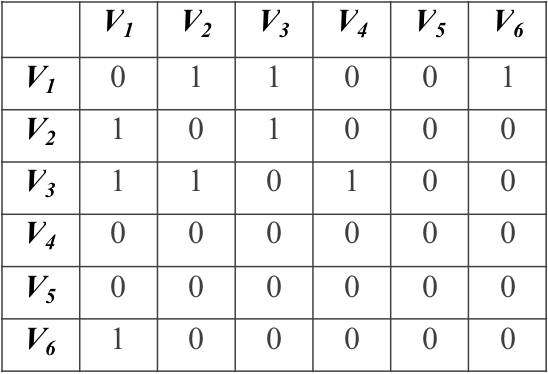
\includegraphics[width=\linewidth/2]{figures/grafos/representacao_matriz_adj.png}
\end{center}

\subsubsection{Lista de Adjacência}

\indent\indent A lista de adjacência se baseia em guardar, para cada vértice, quais são os seus vizinhos, ou, de uma maneira geral, guardar as arestas que partem desse vértice.

\indent O uso da lista de adjacência pode ser complicado de implementar e debugar para pessoas iniciantes, mas acaba sendo a representação mais usada por pessoas experientes. Isso se deve ao fato de a lista de adjacência possuir complexidade O(1) para inserir novas arestas e um tempo otimizado para consultas num único vértice.

\indent A representação do grafo por lista de adjacência fica da seguinte maneira:

\begin{center}
  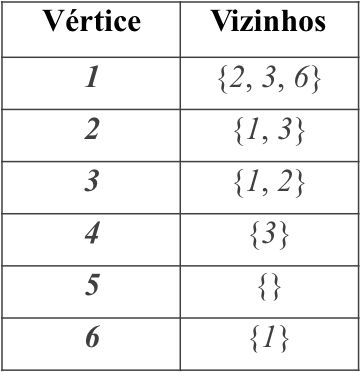
\includegraphics[width=\linewidth/2]{figures/grafos/representacao_lista_adj.png}
\end{center}

\end{document}